\documentclass{article} % For LaTeX2e
\usepackage{nips13submit_e,times}
\usepackage{hyperref}
\usepackage{url}
\usepackage{lipsum}
\usepackage{float}
\usepackage{listings}
\usepackage[pdftex]{graphicx} 
%\documentstyle[nips13submit_09,times,art10]{article} % For LaTeX 2.09


\title{A Twitter-Based Climate Change Stance Classification Pipeline}


\author{
Jiarong Ye\\
College of Engineering\\
\texttt{jxy225@psu.edu} \\
\And
Yuan Meng\\
College of Information Science and Technology\\
\texttt{yfm5047@psu.edu} \\
}



\newcommand{\fix}{\marginpar{FIX}}
\newcommand{\new}{\marginpar{NEW}}

\nipsfinalcopy % Uncomment for camera-ready version

\begin{document}


\maketitle

\begin{abstract}
The goal of the mini project is to get a hands-on personal experience regarding the construction, interpretation, refinement, deployment, and evaluation of a twitter-based stance classification pipeline.
\end{abstract}

\section{Introduction}

The project is to use one unlabeled dataset which we later tagged by designing our own labeling strategy with crowd-sourced stances and one labeled dataset to construct and improve a model that can predict sentiments of tweets about climate change. The model is able to discriminate if one tweet is supporting for the topic of climate change or not. 

\section{Data Preparation}

Two datasets are used in the project. DS1 is the unlabeled set, so we design a label aggregation strategy on the original 3 labels collected from crowd-sourcing to put a binary label (supportive as 1, non-supportive as 0) on it. It is the dataset that we use for constructing the basic model. DS2 is the labeled set. As the logic of labeling supportive level is not same as the previous one, both datasets have some differences. The combination of DS1 and DS2 is used to improve the model.


\section{Label Aggregation}

The logic to determine the stance of each tweet: 

\begin{itemize}
	\item  First, assign numerical numbers to  different sentiment
	\begin{itemize}
		\item[*] 1 for positive
		\item[*] 0 for neutral
		\item[*] -1 for negative
		\item[*] -2 for irrelevant
	\end{itemize}
	\item  Second, add up three numbers for each tweet
	\item  Third, if the result $\ge$ 1, the tweet is Support; Otherwise, it is Non-Support
\end{itemize}



\section{Model Construction}

Using the set of provided tweets (which have been tagged) to construct two Decision Tree based predictive models predicting whether a tweet is supportive or lack of support for the topic.

\subsection{Baseline Model (Model B: trained by DS1)}

\subsubsection{Dataset}
After we aggregate the labels, DS1 has 716 supporting tweets and 567 non-supporting tweets. It is not too unbalanced, so it can avoid the result being overfitting to the label with significantly larger volume than other labels to some extent.


\subsubsection{Parameters}

\lstset{language=Python}
\lstset{showstringspaces=false}
\lstset{frame=lines}
\lstset{caption={parameters of baseline model}}
\lstset{basicstyle=\footnotesize}
\begin{lstlisting}
* CountVector
	* token_pattern='(([#@]|[0-9]|[a-z]|[A-Z])+)'
	* analyzer = 'word'
	* min_df = 3
* DecisionTree
	* criterion='entropy'
	* max_depth = 7
	* min_samples_leaf = 2
\end{lstlisting}


\subsubsection{Pipeline}

\lstset{language=Python}
\lstset{frame=lines}
\lstset{caption={Model 1 (DS1)}}
\lstset{basicstyle=\footnotesize}
\begin{lstlisting}
clf = Pipeline(
		[('vect', CountVectorizer(token_pattern='(([#@]|[0-9]|[a-z]|[A-Z])+)',
					analyzer = 'word',
					min_df = 3)),
		('clf', DecisionTreeClassifier(criterion='entropy',
					random_state = 100,
					max_depth = 7,
					min_samples_leaf = 2))
		])
\end{lstlisting}



\subsection{Improved Model (Model A: trained by DS1+DS2)}

The improvements of the following parameters of the Baseline Model were implemented:



\subsubsection{Dataset}

Besides DS1, a new dataset is added into the training phase. DS2 has 800 supporting tweets and 800 non-supporting tweets. It is perfectly balanced, which is good for modeling.


\subsubsection{Token Pattern}

By designing a new regular expression as \textbf{token\_pattern} in sklearn CountVectorizer to extract words, usernames and hashtags from the raw tweets, we are aiming to output the feature displayed in each node of the decision tree with better interpretability.

\hyperref[token:tuple]{tree1}
\lstset{language=Python}
\lstset{frame=lines}
\lstset{caption={Previous token pattern}}
\lstset{basicstyle=\footnotesize}
\begin{lstlisting}
* Baseline Model
	* token_pattern="(([#@]|[0-9]|[a-z]|[A-Z])+)" 
\end{lstlisting}

\hyperref[token:word]{tree2}
\lstset{language=Python}
\lstset{frame=lines}
\lstset{caption={Adjusted token pattern}}
\lstset{basicstyle=\footnotesize}
\begin{lstlisting}	
* Improved Model
	* token_pattern="(?!RT|rt|\d+)[@#]*[\w\'_-]{2,100}"
\end{lstlisting}




\subsubsection{Max Depth}

We tried the max depth 1-15 of tree to enhance the model. The F1 Score is list in Table1 and Table 2. By comparing every f1 score, we decide to assign 15 as the max\_depth for our final decision tree.


\subsubsection{N-Gram}

We change the n-gram parameter when constructing word dictionary as well to include not just single words but also phrases into consideration for the feature set.

\lstset{language=Python}
\lstset{frame=lines}
\lstset{caption={Adjusted n-gram}}
\lstset{basicstyle=\footnotesize}
\begin{lstlisting}	
* Improved Model
	* n-gram=(1,2)
\end{lstlisting}

\subsubsection{Stop Words}

\textbf{Option 1:}

default ('english')

\begin{table}[H]
	\caption{F1 Score}
	\label{sample-table}
	\begin{center}
		\begin{tabular}{|l|l|l|}
			\multicolumn{1}{c}{\bf Max Depth}  
			&\multicolumn{1}{c}{\bf Test Set}
			&\multicolumn{1}{c}{\bf Train Set}
			\\ \hline & &  \\
			1        &0.690 &0.597	 \\
			2        &0.688	&0.682	  \\
			3        &0.684	&0.688	 \\
			4        &0.693	&0.697	 \\
			5        &0.693	&0.703 \\
			6        &0.693 &0.706   \\
			7        &0.694 &0.711   \\
			8        &0.682 &0.714   \\
			9        &0.704 &0.718    \\
			10       &0.693  &0.719    \\
			11       &0.677  &0.723   \\
			12       &0.688 &0.728  \\
			13       &0.683 &0.733  \\
			14       &0.677  &0.736  \\
			15       &0.672 &0.735  \\
			\hline
		\end{tabular}
	\end{center}
\end{table}


\begin{figure}[H]
	\centering
	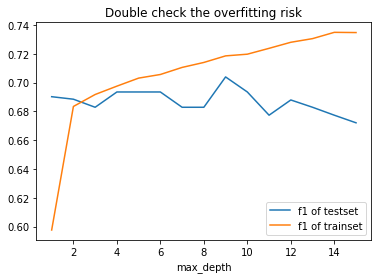
\includegraphics[height=6cm, width=8cm]{2.png}
	\caption{F1 score of training and testing set}
\end{figure}


\textbf{Option 2: }

self-defined: {'a', 'an', 'the', 'it', 'is', 'are', 'be', 'of', 'this', 'that', 'RT', 'rt','https'}


\begin{table}[H]
	\caption{F1 Score}
	\label{sample-table}
	\begin{center}
		\begin{tabular}{|l|l|l|}
			\multicolumn{1}{c}{\bf Max Depth}  
			&\multicolumn{1}{c}{\bf Test Set}
			&\multicolumn{1}{c}{\bf Train Set}
			\\ \hline & &  \\
			1        &0.479 &0.605	 \\
			2        &0.648	&0.683	  \\
			3        &0.672	&0.698	 \\
			4        &0.660	&0.702	 \\
			5        &0.637	&0.706 \\
			6        &0.631 &0.714   \\
			7        &0.649 &0.721   \\
			8        &0.650 &0.721   \\
			9        &0.631 &0.724    \\
			10       &0.693  &0.719    \\
			11       &0.620  &0.731   \\
			12       &0.631 &0.739  \\
			13       &0.621 &0.747  \\
			14       &0.596 &0.749  \\
			15       &0.614 &0.748  \\
			\hline
		\end{tabular}
	\end{center}
\end{table}


\begin{figure}[H]
	\centering
	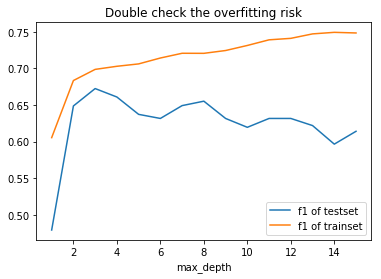
\includegraphics[height=7cm, width=8cm]{3.png}
	\caption{F1 score of training and testing set}
\end{figure}


\textbf{Option 3$^*$:}

The top 30 most common words in DS1+DS2 tweets (exclude semantic sensitive words like \textbf{climate} and \textbf{change})

\lstset{language=Python}
\lstset{frame=lines}
\lstset{caption={Get the words with the highest frequency}}
\lstset{basicstyle=\footnotesize}
\begin{lstlisting}
stop_w = [i[0] for i in Counter([word for sentence in X for word in sentence.split() 
		if 'climate' not in word.lower() and 'change' not in word.lower()
		and word.isalpha() 
		and len(word)>1]).most_common()[:30]]

output: 
	['the', 'to', 'RT', 'of', 'is',	'and','in', 'that', 'on', 'for', 'are',	'you', 
	'we', 'The', 'it', 'this', 'about', 'be', 'by', 'have', 'not', 'will', 'our', 
	'from', 'as', 'with', 'can', 'all', 'We', 'do']
\end{lstlisting}



\begin{table}[H]
	\caption{F1 Score}
	\label{sample-table}
	\begin{center}
		\begin{tabular}{|l|l|l|}
			\multicolumn{1}{c}{\bf Max Depth}  
			&\multicolumn{1}{c}{\bf Test Set}
			&\multicolumn{1}{c}{\bf Train Set}
			\\ \hline & &  \\
			1        &0.647 &0.599	 \\
			2        &0.708	&0.683	  \\
			3        &0.690	&0.693	 \\
			4        &0.700	&0.699	 \\
			5        &0.701	&0.707 \\
			6        &0.701 &0.712   \\
			7        &0.684 &0.717   \\
			8        &0.690 &0.717   \\
			9        &0.690 &0.721    \\
			10       &0.724  &0.729    \\
			11       &0.719  &0.733   \\
			12       &0.714 &0.735  \\
			13       &0.708 &0.741  \\
			14       &0.714 &0.740  \\
			15       &0.702 &0.745  \\
			\hline
		\end{tabular}
	\end{center}
\end{table}



\begin{figure}[H]
	\centering
	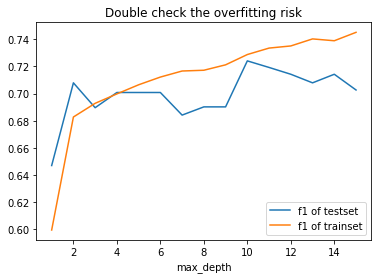
\includegraphics[height=7cm, width=8cm]{4.png}
	\caption{F1 score of training and testing set}
\end{figure}



\subsubsection{Pipeline}

\lstset{language=Python}
\lstset{frame=lines}
\lstset{caption={Model 2 (DS2)}}
\lstset{basicstyle=\footnotesize}
\begin{lstlisting}
stop_w = [i[0] for i in Counter([word for sentence in X 
		for word in sentence.split() 
		if 'climate' not in word.lower() and 'change' not in word.lower()
		and word.isalpha() 
		and len(word)>1]).most_common()[:30]]

output: 
	['the', 'to', 'RT', 'of', 'is',	'and','in', 'that', 'on', 'for', 'are',	'you', 
	'we', 'The', 'it', 'this', 'about', 'be', 'by', 'have', 'not', 'will', 'our', 
	'from', 'as', 'with', 'can', 'all', 'We', 'do']

clf = Pipeline(
	[('vect',CountVectorizer(token_pattern="(?!RT|rt|\d+)[@#]*[\w\'_-]{2,100}",
				analyzer = 'word',
				stop_words = stop_w,
				min_df = 10,
				ngram_range=(1,2))),
	('clf', DecisionTreeClassifier(criterion='entropy',
				random_state = 100,
				max_depth = 15,
				min_samples_leaf = 2))
	])
\end{lstlisting}


\section{Model Assessment}

\subsection{Baseline Model (Model B: trained by DS1)}

\begin{table}[H]
	\caption{5-fold output of decision tree with max\_path=7, min\_samples\_leaf=2}
	\label{sample-table}
	\begin{center}
		\begin{tabular}{|l|l|l|l|l|}
			\multicolumn{1}{c}{\bf Fold}  
			&\multicolumn{1}{c}{\bf Accuracy}
			&\multicolumn{1}{c}{\bf Precision} 
			&\multicolumn{1}{c}{\bf Recall}
			&\multicolumn{1}{c}{\bf F1 score}
			\\ \hline & & & & \\
			1	&0.639535	&0.649123	&0.770833	&0.704762 \\
			2	&0.649805	&0.680272	&0.699301	&0.689655 \\
			3	&0.589844	&0.613095	&0.720280	&0.662379 \\ 
			4	&0.593750	&0.610169	&0.755245	&0.675000  \\
			5	&0.601562	&0.627329	&0.706294	&0.664474  \\
			\hline
		\end{tabular}
	\end{center}
\end{table}


We check overfitting risk by comparing the model's confusion matrix for training data vs the model's confusion matrix for testing data based on max\_path=7, min\_samples\_leaf=2 of the decision tree:

\begin{figure}[H]
	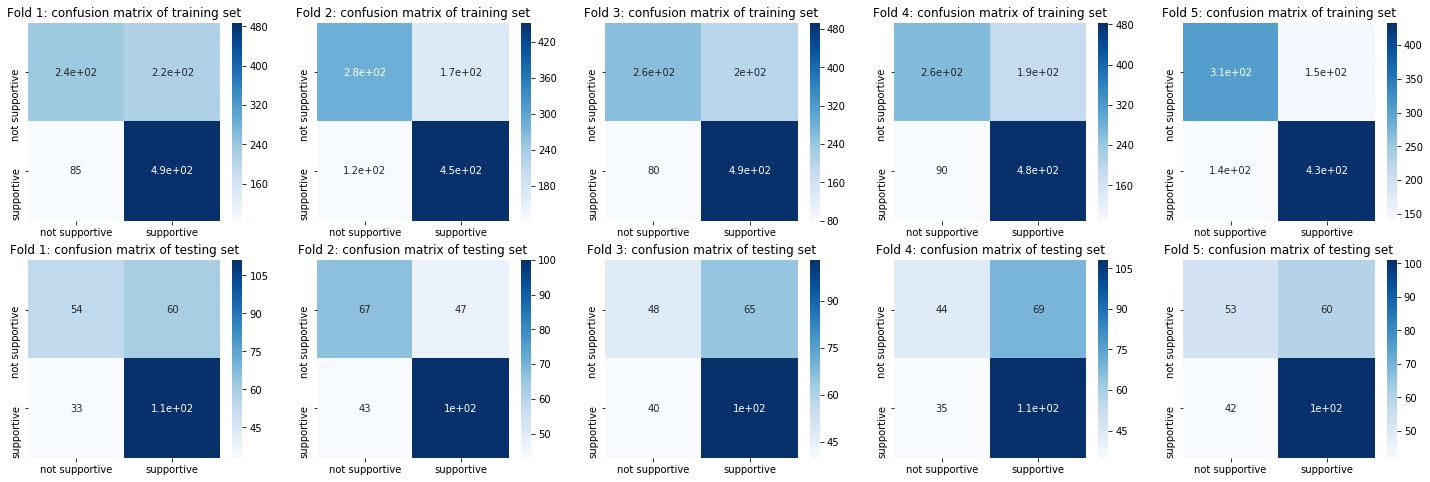
\includegraphics[height=5cm, width=17cm]{5.png}
	\caption{Confusion Matrix of training and testing set to observe overfitting}
\end{figure}



\subsection{Improved Model (Model A: trained by DS1+DS2)}

\begin{table}[H]
	\caption{5-fold output of decision tree with max\_path=15, min\_samples\_leaf=2}
	\label{sample-table}
	\begin{center}
		\begin{tabular}{|l|l|l|l|l|}
			\multicolumn{1}{c}{\bf Fold}  
			&\multicolumn{1}{c}{\bf Accuracy}
			&\multicolumn{1}{c}{\bf Precision} 
			&\multicolumn{1}{c}{\bf Recall}
			&\multicolumn{1}{c}{\bf F1 score}
			\\ \hline & & & & \\
			1        &0.617594	&0.611111	&0.750853	&0.673813 \\
			2        &0.628366	&0.627976	&0.720137	&0.670906 \\
			3        &0.646320	&0.639535	&0.750853	&0.690738 \\
			4        &0.647482	&0.639535	&0.753425	&0.691824 \\
			5        &0.638489	&0.631124	&0.750000	&0.685446 \\
			\hline
		\end{tabular}
	\end{center}
\end{table}

We check overfitting risk by comparing the model's confusion matrix for training data vs the model's confusion matrix for testing data based on max\_path=15, min\_samples\_leaf=2 of the decision tree:

\begin{figure}[H]
	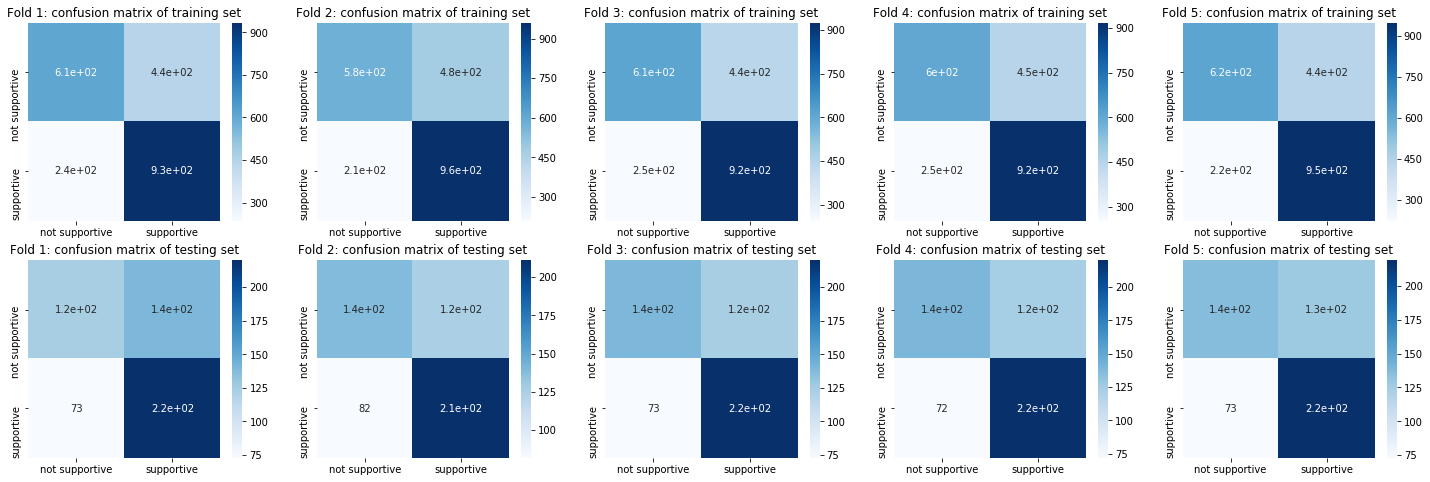
\includegraphics[height=6cm, width=17cm]{1.png}
	\caption{Confusion Matrix of training and testing set to observe overfitting}
\end{figure}

Then we use max\_path=15, min\_samples\_leaf=2 for the decision tree to test the model, and the new data is better than the previous one.


\section{Model Interpretation}

\subsection{Baseline Model (Model B: trained by DS1)}

\label{token:tuple}
\subsubsection{Fold 1}

\begin{figure}[H]
	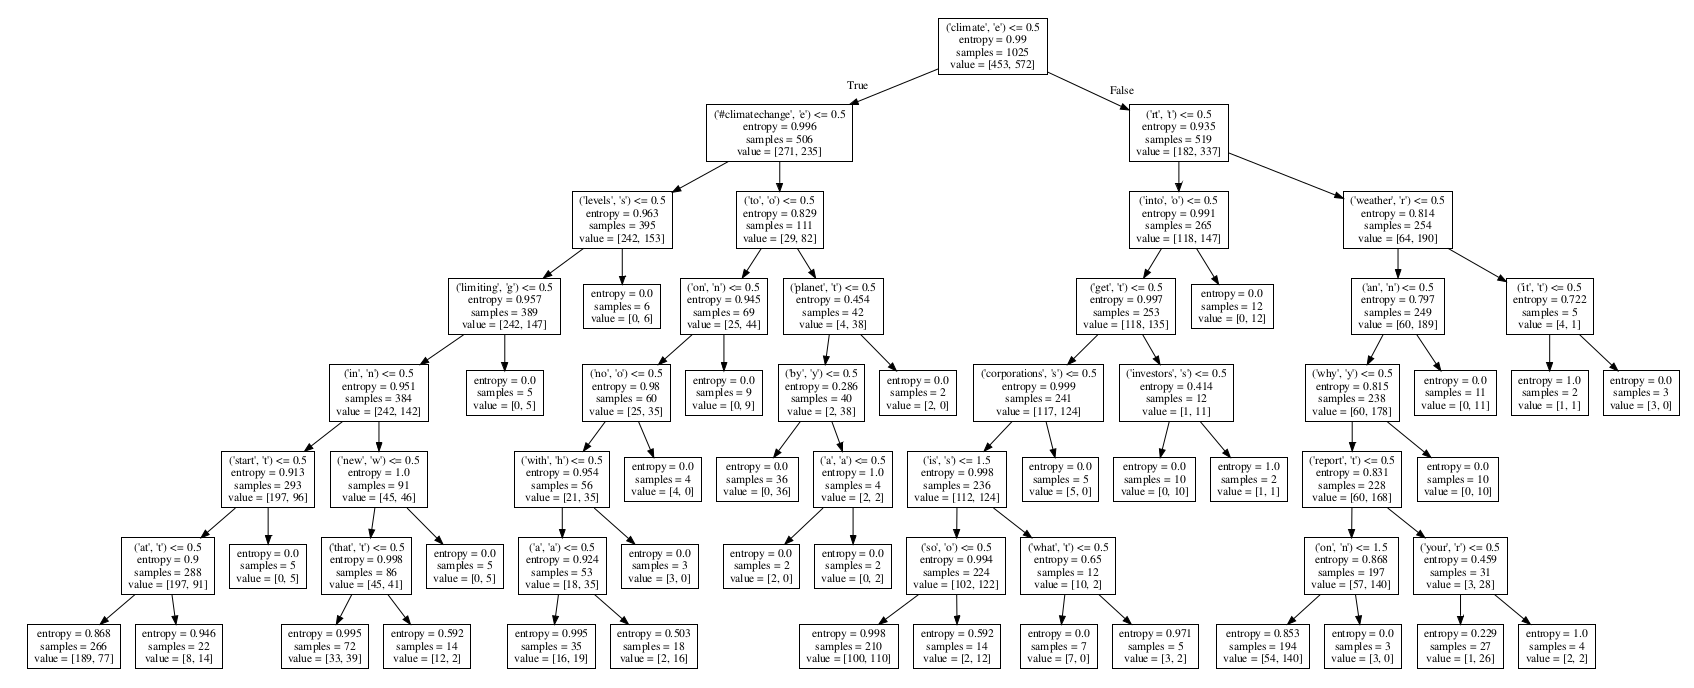
\includegraphics[height=5cm, width=17cm]{6.png}
	\caption{Decision Tree Fold 1 (partial)}
\end{figure}

\subsubsection{Fold 2}

\begin{figure}[H]
	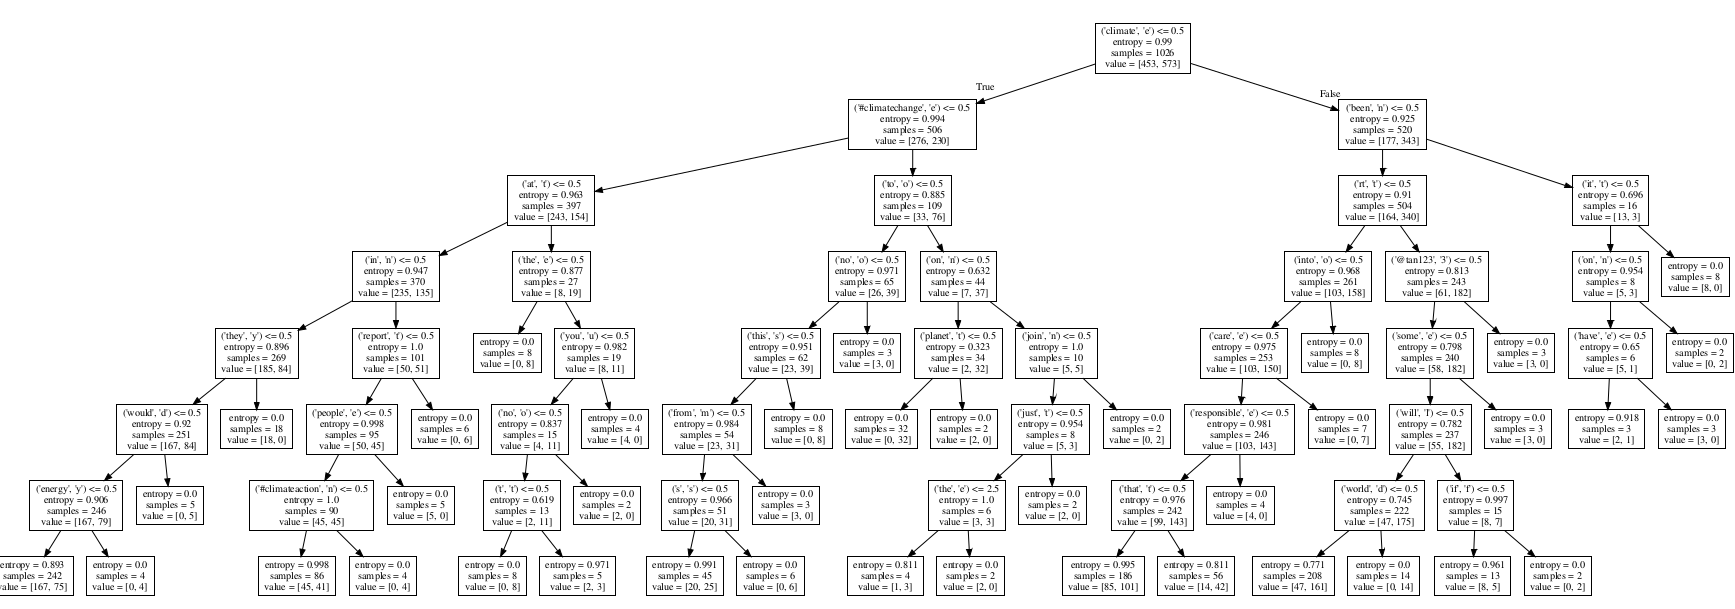
\includegraphics[height=5cm, width=17cm]{7.png}
	\caption{Decision Tree Fold 2 (partial)}
\end{figure}

\subsubsection{Fold 3}

\begin{figure}[H]
	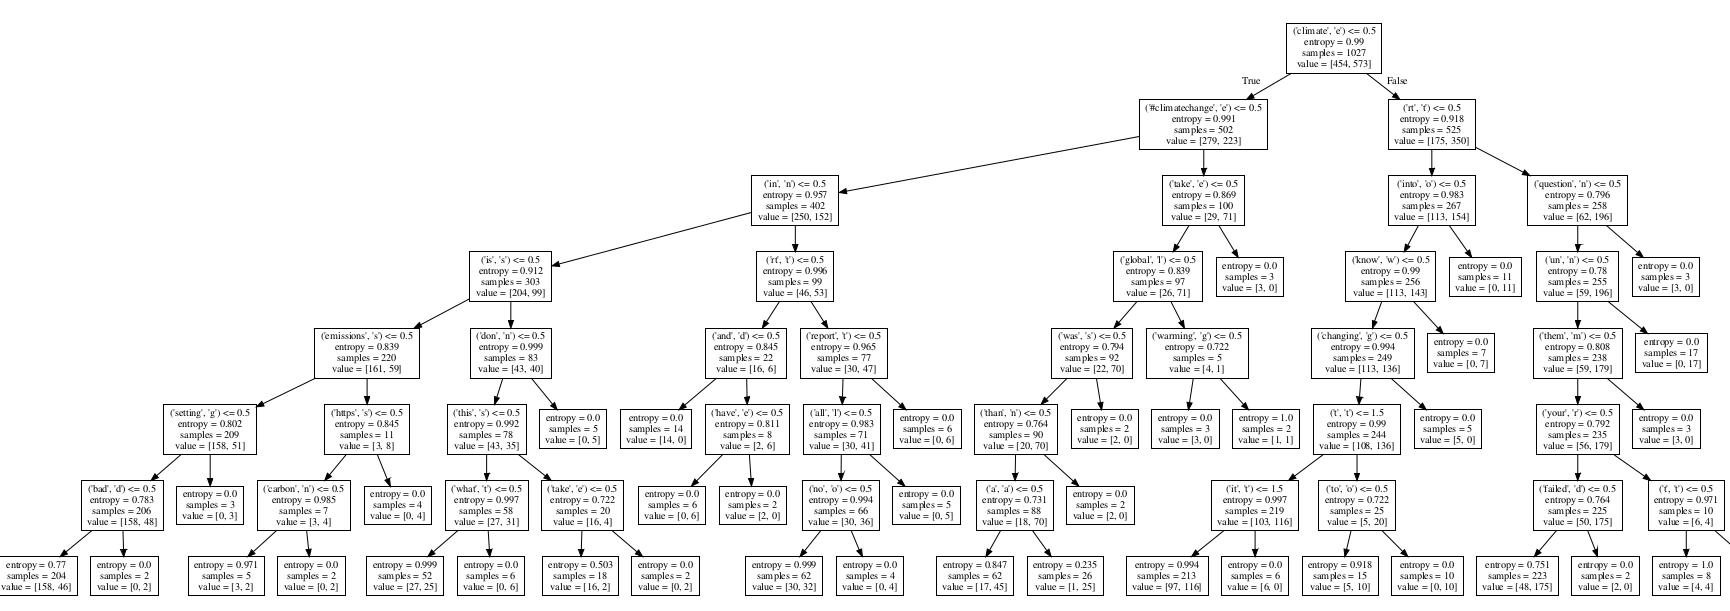
\includegraphics[height=5cm, width=17cm]{8.png}
	\caption{Decision Tree Fold 3 (partial)}
\end{figure}

\subsubsection{Fold 4}

\begin{figure}[H]
	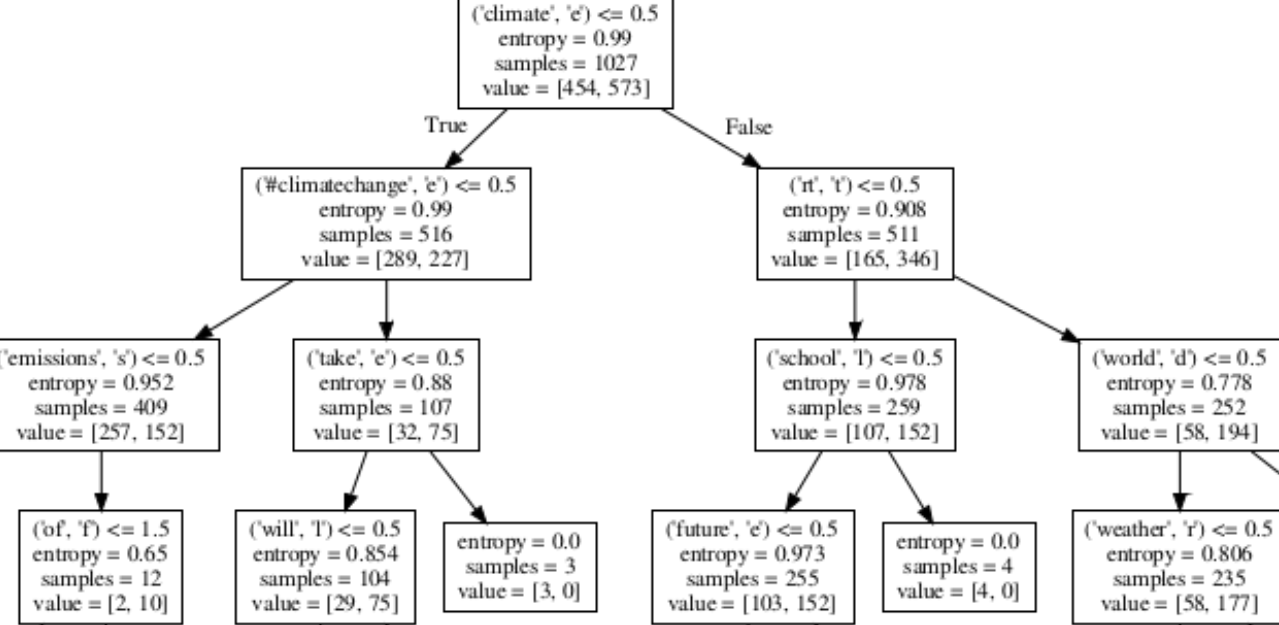
\includegraphics[height=5cm, width=17cm]{9.png}
	\caption{Decision Tree Fold 4 (partial)}
\end{figure}

\subsubsection{Fold 5}

\begin{figure}[H]
	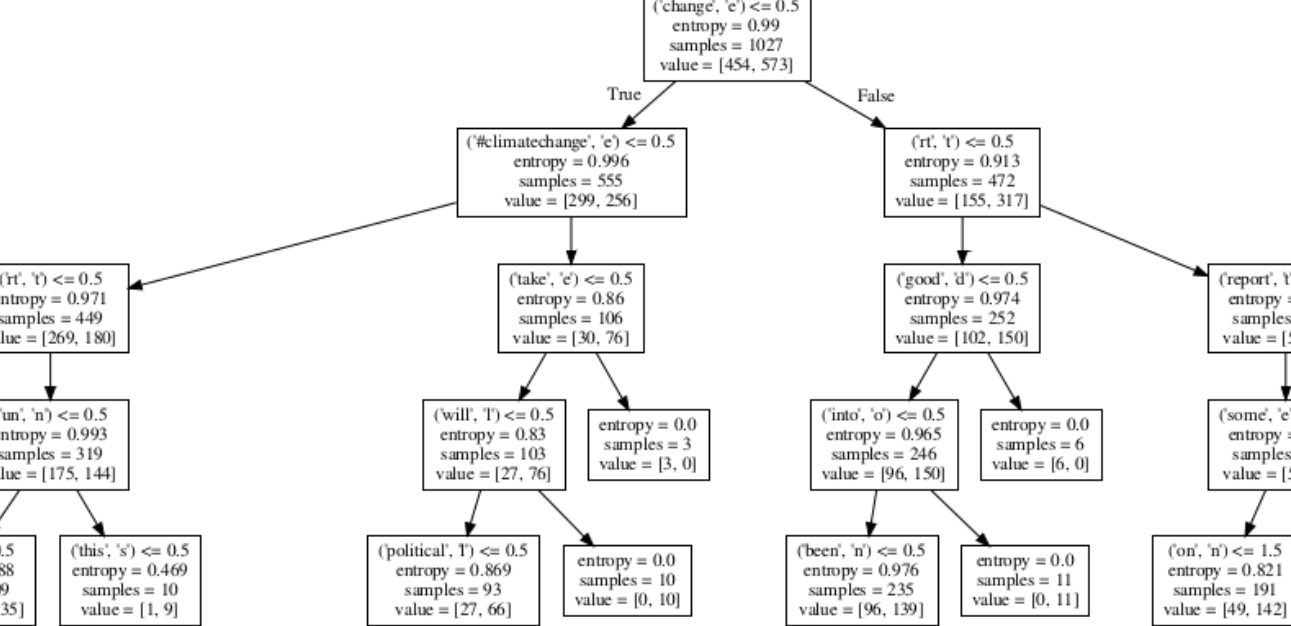
\includegraphics[height=5cm, width=17cm]{10.png}
	\caption{Decision Tree Fold 5 (partial)}
\end{figure}


Rule examples of Baseline Model (Model B: trained by DS1): 
\begin{itemize}
	\item  If a tweet does not contain 'climate', '\#climatechange', but contains 'levels', then it is much more likely to \textbf{SUPPORT} Climate Change.
	\item  If a tweet contains 'climate', 'corporations', but does not contain 'rt', 'into', 'get',  then it is much more likely to \textbf{NOT SUPPORT} Climate Change.
\end{itemize}


\subsection{Improved Model (Model A: trained by DS1+DS2)}


\label{token:word}
\subsubsection{Fold 1}

\begin{figure}[H]
	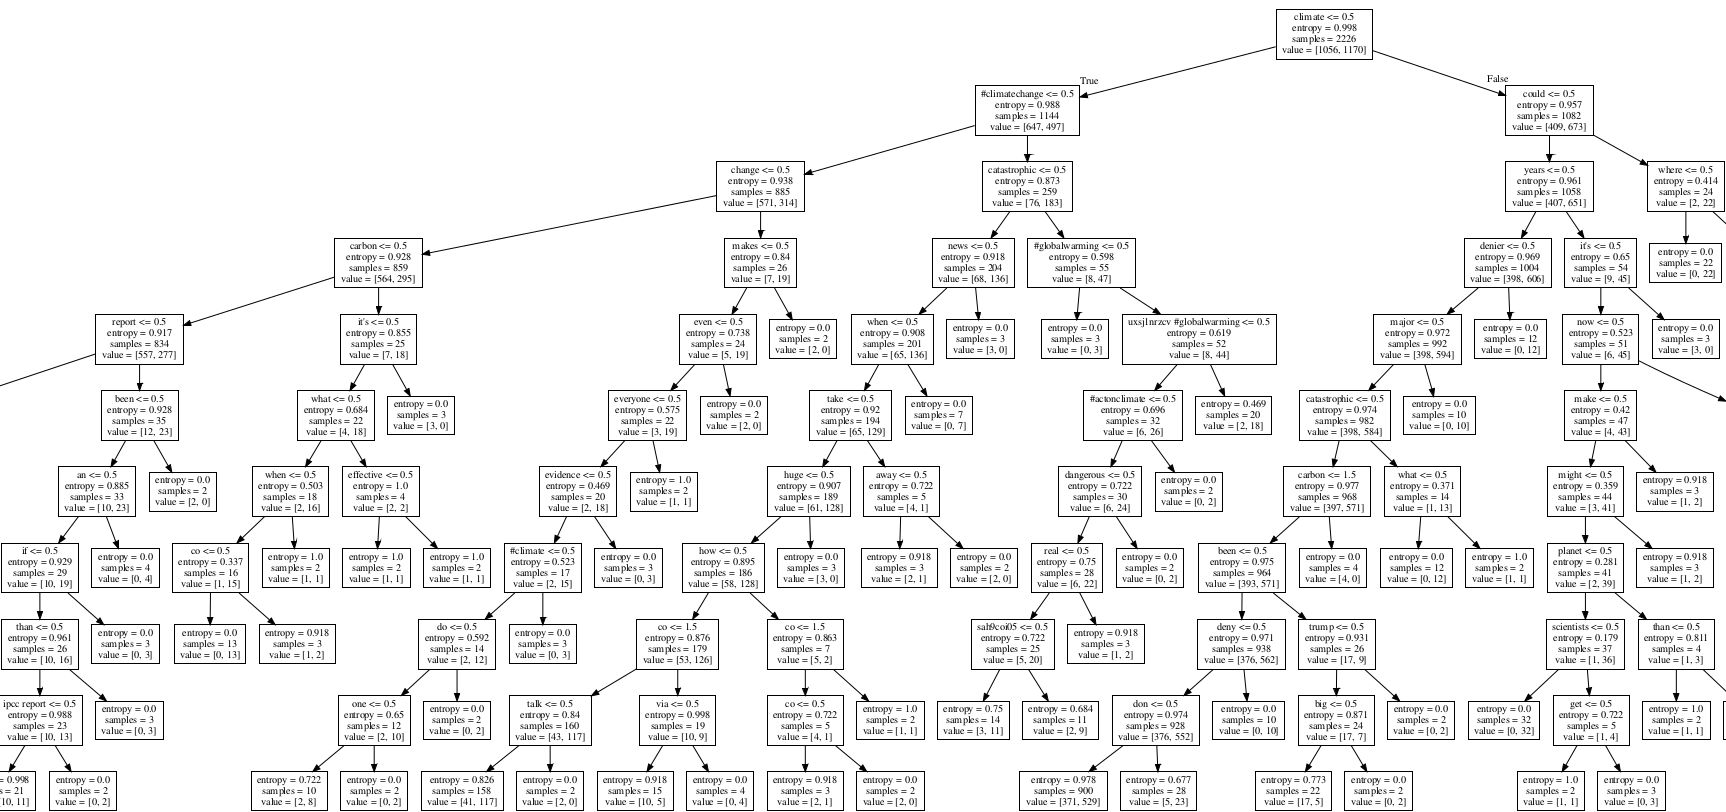
\includegraphics[height=5cm, width=17cm]{11.png}
	\caption{Decision Tree Fold 1 (partial)}
\end{figure}

\subsubsection{Fold 2}

\begin{figure}[H]
	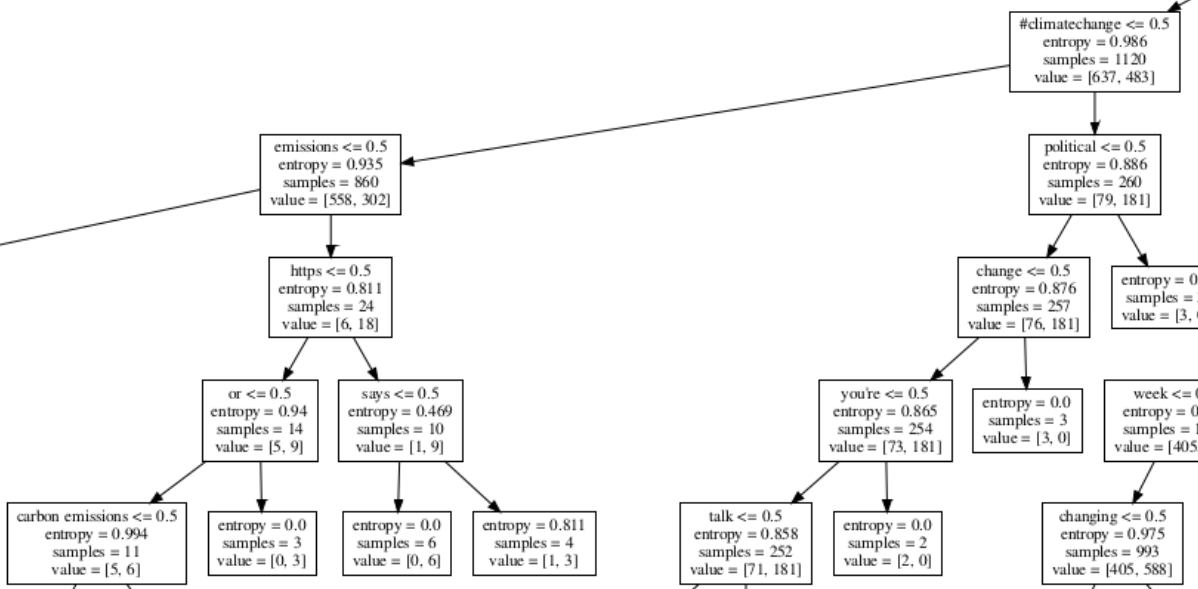
\includegraphics[height=5cm, width=17cm]{12.png}
	\caption{Decision Tree Fold 2 (partial)}
\end{figure}

\subsubsection{Fold 3}

\begin{figure}[H]
	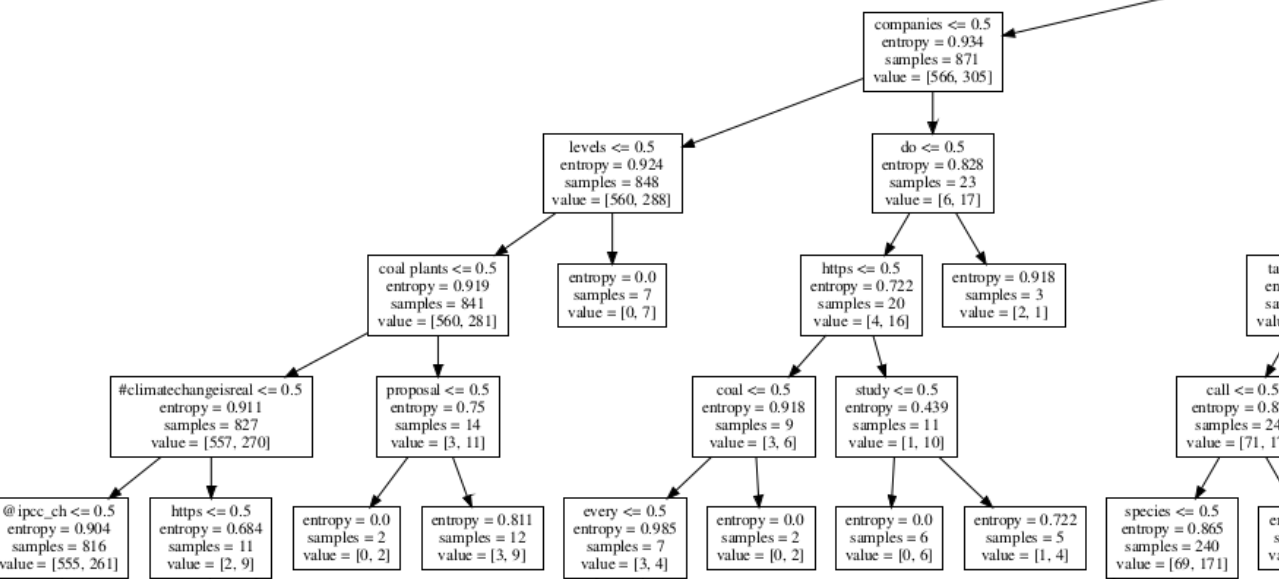
\includegraphics[height=5cm, width=17cm]{13.png}
	\caption{Decision Tree Fold 3 (partial)}
\end{figure}

\subsubsection{Fold 4}

\begin{figure}[H]
	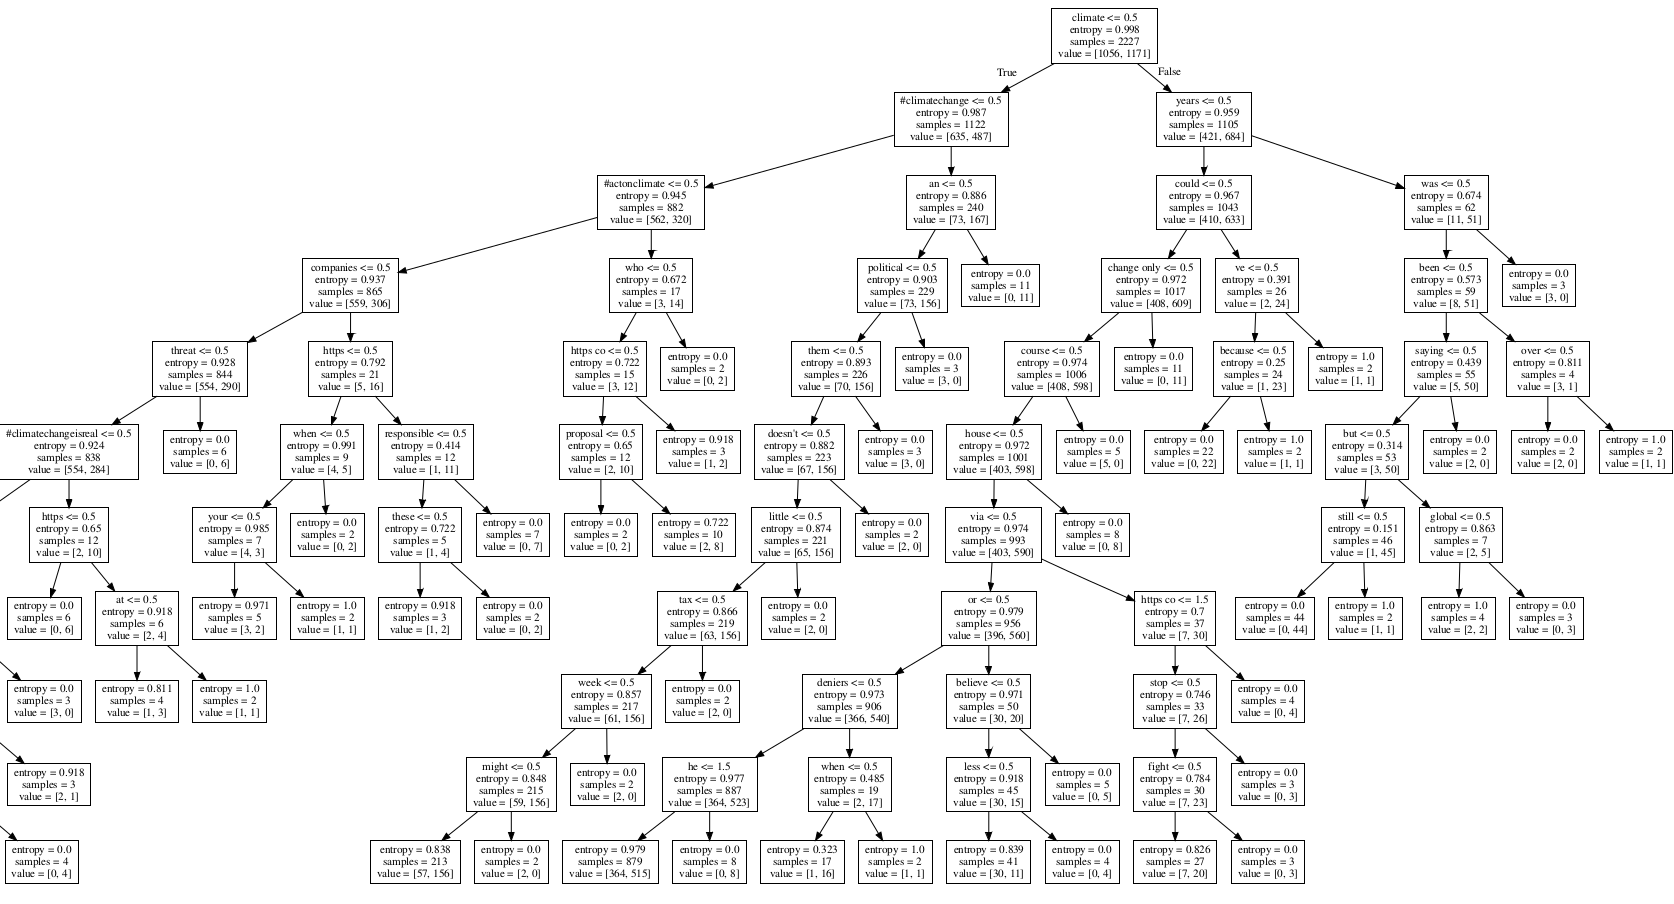
\includegraphics[height=5cm, width=17cm]{14.png}
	\caption{Decision Tree Fold 4 (partial)}
\end{figure}

\subsubsection{Fold 5}

\begin{figure}[H]
	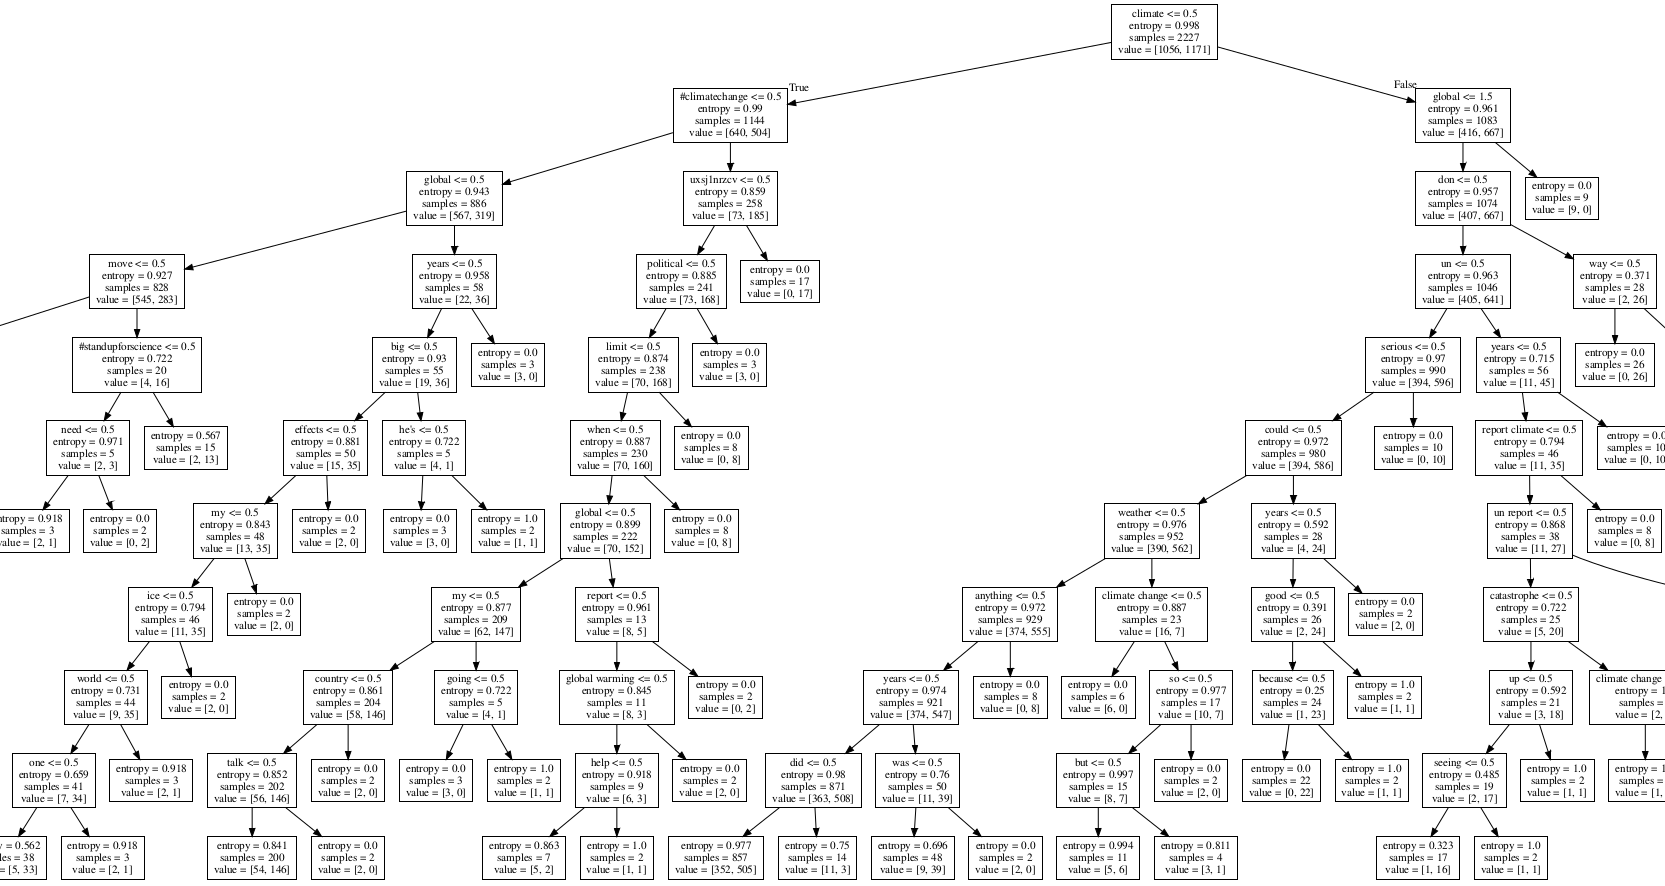
\includegraphics[height=5cm, width=17cm]{15.png}
	\caption{Decision Tree Fold 5 (partial)}
\end{figure}

\textit{Note$^*$: The improved decision tree does not have unmeaningful nodes such as \textbf{"rt/RT"}, and its max depth is deeper than the original one.}

Rule examples of Improved Model: 
\begin{itemize}
	\item If a tweet does not contain 'climate', '\#climatechange', 'change', 'carbon', 'been', 'an', but contains 'respond', 'if', then it is much more likely to \textbf{SUPPORT} Climate Change.
	\item If a tweet contains 'climate', 'years', but does not contain 'could', 'it's', 'now', 'make', 'might', 'planet', 'scientists', then it is much more likely to \textbf{NOT SUPPORT} Climate Change.
\end{itemize}





\section{Conclusion/Future Work}


We generated two models during the progress of the project. Model A is trained with the combination of DS1 and DS2, and Model B is only trained with DS1. We have Model B first, then we improve the model and get Model A. 

In retrospective, there are several lessons we learned throughout the implementation of the twitter-based project, which is like a NLP 101. We got some really useful hands-on experience with the twitter data from first applying for a Twitter developer account, then collecting with a script pipeline written in python, then preprocessing it by dropping all replicates to avoid potential overfitting in the model training phase later and writing regular expressions to extract words, usernames and hashtags ready to build a word dictionary by sklearn CountVectorizer. In the model building step, we got to try setting up a Decision Tree for the stance classification task followed by  a 5-fold cross-validation strategy for model evaluation. We got a decent final result at last.  We change the max depth from 7 to 15, make some adjustments about stop-words, n-grams and the f1 score bumps up from 0.718 to 0.719. In the process, there are a few tips worth mentioning. The stop word is useful for building the decision tree. Some words occur in tweets frequently but they do not contribute for identifying the sentiment of tweets, the usage of stop words helps prevent words such as "rt" or "the" from appearing in the trees. We forget to change the min\_sample\_leaf of the tree to get the better score, this is the lesson we should learn.
 
For future endeavor, there are a lot of word-encoding strategies and classifiers to examine for the twitter binary stance classification task, for instance, besides count-based bag-of-words, tf-idf \cite{scikit-learn} could also be considered as an alternative (however, since the fact that the word count of each tweet is limited, tf-idf might not works as well as it does for similar binary sentiment classification trained by documents as corpus, in which case vectorized by tf-idf could reduce the over-sparsity of the feature set significantly). Besides statistical measured word encoding approaches, pre-trained Glove \cite{glove} or Word2Vec \cite{w2v} for twitter corpus is worthing trying out as well regarding text encoding. And for the binary classifier, to improve the f1 score with tree-based algorithm, we could try the ensemble method as a combination of multiple weak learners, for instance, Random Forest \cite{scikit-learn}, AdaBoosting \cite{scikit-learn}, XGBoost \cite{xg}, despite the major drawback as comprising the interpretability of the decision rules.

\[\]


\section{Appendix}
\appendix
\section{Python Code}

\lstset{language=Python}
\lstset{frame=lines}
\lstset{caption={import packages}}
\lstset{basicstyle=\footnotesize}
\begin{lstlisting}
import datascience as ds
from datascience import *
import numpy as np
from collections import Counter
from graphviz import Source
import pandas as pd
import seaborn as sns
from sklearn.pipeline import Pipeline
from sklearn.feature_extraction.text import CountVectorizer, TfidfTransformer
from sklearn.tree import DecisionTreeClassifier
from sklearn.ensemble import RandomForestClassifier
from sklearn import tree
from sklearn.metrics import confusion_matrix, precision_score, recall_score, f1_score, 
			    accuracy_score, classification_report
import matplotlib.pyplot as plt
from sklearn.model_selection import train_test_split, cross_val_score, StratifiedKFold
from sklearn.externals import joblib
%matplotlib inline
\end{lstlisting}


\lstset{language=Python}
\lstset{frame=lines}
\lstset{caption={Aggregate supportive/non-supportive Label}}
\lstset{basicstyle=\footnotesize}
\begin{lstlisting}
df = pd.read_csv(filepath, sep=',')

def aggregate_labels(df, agg_label, support_level):
	labels = df.columns[2:]
	for label in labels:
		for key, val in STANCE_VAL_DICT.items():
	df[label] = df[label].replace(key, val)
	df[agg_label] = df[df.columns[2:]].apply(lambda x: np.sum(x.values), axis=1)
	df[support_level] = df.iloc[:, -1].apply(lambda x: 1 if x>=1 else 0)
	df = df.drop(columns=df.columns[2:6])
	supportive_cnt = df.loc[df[support_level]==1, :].shape[0]
	unsupportive_cnt = df.loc[df[support_level]==0, :].shape[0]
	df.to_csv('Climate1SupportiveLevel.csv')

aggregate_labels(df, 'FinalLabel', 'SupportiveLabel')
\end{lstlisting}


\lstset{language=Python}
\lstset{frame=lines}
\lstset{caption={Combine DS1 and DS2 and randomly extract 100 tweets for final testing}}
\lstset{basicstyle=\footnotesize}
\begin{lstlisting}
df1 = ds.Table.read_table('Climate1SupportiveLevel.csv', sep=',')
df2 = ds.Table.read_table('ClimateBalancedDS2.csv', sep=',')
df = df1.append(df2)
test_index = np.random.choice(df.num_rows, 100, replace=False)
train_val_index = [i for i in np.arange(df.num_rows) if i not in test_index]
test_data = df.take[test_index]
df = df.take[train_val_index]
X = list(df['Text'])
y = list(df['Support'])
test_X = list(test_data['Text'])
test_y = list(test_data['Support'])
\end{lstlisting}


\lstset{language=Python}
\lstset{frame=lines}
\lstset{caption={Check whether the data distribution is balanced}}
\lstset{basicstyle=\footnotesize}
\begin{lstlisting}
def check(sentiment, index, note='training'):
	if sentiment==0:
		label = 'not supportive'
	else:
		label = 'supportive'
	print('There are {} '.format(df.take(index).where('Support', 
		are.equal_to(sentiment)).size[0][0])+label+' tweets in the '+note+' set.')
\end{lstlisting}

\lstset{language=Python}
\lstset{frame=lines}
\lstset{caption={Split data into training and validation dataset}}
\lstset{basicstyle=\footnotesize}
\begin{lstlisting}
def custom_split(train_index, test_index):
	trainingset = df.take(train_index)
	testingset = df.take(test_index)    
	
	X_train= list(trainingset['Text'])
	y_train= list(trainingset['Support'])
	X_test= list(testingset['Text'])
	y_test= list(testingset['Support'])
	
	return X_train, X_test, y_train, y_test
\end{lstlisting}



\lstset{language=Python}
\lstset{frame=lines}
\lstset{caption={Classifier}}
\lstset{basicstyle=\footnotesize}
\begin{lstlisting}
def classifier(X_train, y_train, X_test, fold, max_depth, min_samples_leaf):
	clf = Pipeline(
		[('vect', CountVectorizer(token_pattern="(?!RT|rt|\d+)[@#]*[\w\'_-]{2,100}",
			analyzer = 'word',
			stop_words = 'english',
			min_df = 10,
			ngram_range=(1,2))),
		('clf', DecisionTreeClassifier(criterion='entropy',
			random_state = 100,
			max_depth = max_depth,
			min_samples_leaf = min_samples_leaf))
		])
	clf.fit(X_train, y_train)
	feature_names = clf.named_steps['vect'].get_feature_names()
	try:
		dot_data = tree.export_graphviz(clf.named_steps['clf'], out_file=None, 
		feature_names=feature_names)
		graph = Source(dot_data)
		graph.render('ClimateClassifier-Fold_{}'.format(fold))
	except Exception as e:
		print(e)
	predicted_y_train = clf.predict(X_train)
	predicted_y_test = clf.predict(X_test)
	# save as pickle
	joblib.dump(clf, 'ClimateTeam7PD2.pkl')
	return predicted_y_train, predicted_y_test
\end{lstlisting}


\lstset{language=Python}
\lstset{frame=lines}
\lstset{caption={Evaluation Metrics}}
\lstset{basicstyle=\footnotesize}
\begin{lstlisting}
def eval_results(predicted_y_train, y_train, predicted_y_test, y_test, fold):
	accuracy_s = accuracy_score(y_test, predicted_y_test)
	precision_s = precision_score(y_test, predicted_y_test)
	recall_s = recall_score(y_test, predicted_y_test)
	f1_s = f1_score(y_test, predicted_y_test)
	cm_train = confusion_matrix(y_train, predicted_y_train)
	cm_test = confusion_matrix(y_test, predicted_y_test)  
	
	print('Accuracy Score:', accuracy_s)
	print("Precision Score:", precision_s)
	print("Recall Score:", recall_s)
	print("f1 Score:", f1_s)
	print('confusion_matrix of training set is: \n', cm_train, '\n')
	print('confusion_matrix of testing set is: \n', cm_test, '\n')
	print(classification_report(y_test, predicted_y_test))
	
	classes = ['not supportive', 'supportive']
	plt.subplot(2, 5, fold)
	sns.heatmap(cm_train, annot=True, cmap='Blues', yticklabels=classes, 
							xticklabels=classes)
	plt.title('Fold {}: confusion matrix of training set'.format(fold))
	plt.subplot(2, 5, fold+5)
	sns.heatmap(cm_test, annot=True, cmap='Blues', yticklabels=classes, 
						 	xticklabels=classes)
	plt.title('Fold {}: confusion matrix of testing set'.format(fold))
	return accuracy_s, precision_s, recall_s, f1_s
\end{lstlisting}


\lstset{language=Python}
\lstset{frame=lines}
\lstset{caption={Training with K-fold cross validation}}
\lstset{basicstyle=\footnotesize}
\begin{lstlisting}
def k_fold_evaluate(X, y, max_depth, min_samples_leaf, stop_words,
				print_eval=True, overfit_risk=False):
	# initialization
	accuracy = []
	precision = []
	recall=[]
	f1 = []
	fold = 1
	skf = StratifiedKFold(n_splits=5, random_state=1, shuffle= True)

	# build model and collect results
	for val_index, test_index in skf.split(X, y):
		X_train, X_val, y_train, y_val = custom_split(val_index, test_index)

		predicted_y_train, predicted_y_val = classifier(
							X_train=X_train,
							y_train=y_train, 
							X_test=X_val, fold=fold,
							max_depth = max_depth,
							min_samples_leaf = min_samples_leaf,
							stop_words = stop_words,
							overfit_risk=overfit_risk)
		metrics_df={}
		if print_eval:
			print('\nFold: {}'.format(fold))
			accuracy_s, precision_s, recall_s, f1_s =
			 eval_results(predicted_y_train, y_train, predicted_y_val, y_val)
			
			accuracy.append(accuracy_s)
			precision.append(precision_s)
			recall.append(recall_s)
			f1.append(f1_s)
			
			metrics_df = pd.DataFrame(
			{
				'accuracy': accuracy,
				'precision': precision,
				'recall':recall,
				'f1':f1
			})
		fold += 1
	return metrics_df
\end{lstlisting}


\lstset{language=Python}
\lstset{frame=lines}
\lstset{caption={Testing}}
\lstset{basicstyle=\footnotesize}
\begin{lstlisting}
f1_lst_test = []
f1_lst_train = []
for d in range(1, 15):
	k_fold_evaluate(X, y, max_depth=d, min_samples_leaf=2, stop_words='english', 
			print_eval=False, overfit_risk=True)
	clf_tmp = joblib.load('ClimateTeam7PD2_maxdepth{}.pkl'.format(d))
	print('maxdepth=', d)
	# test
	y_pred = clf_tmp.predict(test_X)
	print('test f1')
	print(f1_score(y_pred=y_pred, y_true=test_y))
	f1_lst_test1.append(f1_score(y_pred=y_pred, y_true=test_y))
	# train_val
	y_pred = clf_tmp.predict(X)
	print('train f1')
	print(f1_score(y_pred=y_pred, y_true=y))
	f1_lst_train1.append(f1_score(y_pred=y_pred, y_true=y))
\end{lstlisting}

\lstset{language=Python}
\lstset{frame=lines}
\lstset{caption={Final Result}}
\lstset{basicstyle=\footnotesize}
\begin{lstlisting}
k_fold_evaluate(X, y, max_depth=15, min_samples_leaf=2, 
stop_words=stop_w, 
print_eval=True, overfit_risk=False)
clf2 = joblib.load('ClimateTeam7PD2.pkl')
\end{lstlisting}



\bibliographystyle{plain}
\bibliography{ref}


\end{document}
